\chapter{Teorie}

Semestrální práce se zabývá zejména problematikou \acs{MIR}. Popsánou v kapitole\ref{sec:MIR}.
Nabízejí se otázky jak by měla daná animace reagovat na konkrétní děj skladby.
Jakým způsobem navrhnout strukturu algoritmů a co by měly získané parametry ovlivňovat při vytváření animací.

V táto části jsou popsány následující segmenty: Teorie zpracování hudební nahrávky pomocí známých algoritmů. Například důležitým algoritmem je \acs{FFT} (\acl{FFT})
popsaná více v bodě \ref{sec:FFT}, jeho variantý pak v bodech \ref{sec:DFT} a \ref{sec:STFT}.
Nabízené moderní metody strojového učení s využitgím hlubokých neuronových sítí při detekci tempa skladby \ref{sec:Detekce_tempa} a určení žánru \ref{sec:Klasifikace_zanru}.  
Struktura a možnosti systému Spectoda pro generování interaktivních světelných animací je podrobně popsána v bodě \ref{sec:Spectoda}.

\section{MIR - Music information retrieval} \label{sec:MIR}
    Music information retrieval je interdisciplinární vědní obor sostředící se na získávání infromací z hudebních nahrávek.
    Jsou zde kombinovány znalosti mnoha oborů jako jsou muzikologie, psychoakustika, strojové učení, zpracování signálů a další. 
    

    Výstup jeho výzkumu je využíván populárními technologiemi. 
    Jednou z aplikací je personalizované doporučování hudebních skladeb, která se nachází v moderních streamovacích platformách.
    Další využítí je v programech pro mixování hudby používaných diskžokeji k plynulejší práci díky alanýze tempe a klíčových částí skladby.
    Tyto technologie se nachází v mnoha dalších aplikacích a s šířením se digitálního audia jejich důležitost stále poroste.
    
    \subsection{Historie}
    V tomto bodě je napsán souhrn historie MIR z knihy \cite{a_new_companion_to_digital_humanities}.
    \acs*{MIR} se začíná objevovat na přelomu devatenáctého a dvacátého století s příchodem moderních statistických metod.
    Začínají se objevovat pokusy o aplikování statistických metod na hudební partitury.
    Protože ještě nebyly natolik dostupné počítače jednalo se spíše o ruční práci s partiturami a tabularueou.
    Z grafických notací se analyzovaly jejich rysy a specifikovaly charakteristiky hudebního díla.
    S příchodem počítačů do výzkumných laboratoří v letech 1960 až 1970 se začalo více rozvíjet zpracování sginálů a s tím související možnosti analýzy hudebních nahrávek pomocí počítačů.
    V těchto letech se poprvé začaly objevoat nyní známé termíny jako \uv{computational musicology} a \uv{ music information retrieval}
    První oblast výzkumu se soustředila na analazýzu tempa skladby. Z důvodu nízké popularity se však výzkum zpomalil.
    Tento útlum pokračoval až do roku 1990 kdy výzkumu \acs*{MIR} pomohly dvě změny.
    První důležitou změnou byly rostoucí databáze digitální hudby, která se staly lehce dostupné pro výzkumné týmy.
    Druhým bodem který přispěl k vývoji \acs{MIR} byl nárůst výpočetního výkonu počítačů a nižší náklady s nimi spojené.
    Díky těmto změnám se stal výzkum dostupnější a jednodužší na realizaci \cite{a_new_companion_to_digital_humanities}.

    Poté v říjnu roku 2000 bylo uspořádáno první mezinárodní symposium soustředící se na \acs{MIR}.
    Z této mezinárodní konference se stala tradice a vybudovala se kolem ní velká komunita nazývaná \acs{ISMIR}\footnote{International Society of Music Information Retrieval - Mezinárodní sdružení pro \acs*{MIR}}.
    Každoročním vyvrcholením \acs{ISMIR} je právě váše zmíněná konference, na které vědci z celého světa prezentují pokroky v oblasti výzkumu \acs{MIR}.
    Zanedlouho naté v roce 2005 byl v rámic této konference představen model \acs{MIREX}\footnote{The Music Information Retrieval Evaluation eXchange - komunitní rámec pro hodnocení pokroků výzkumu v oblasti \acs{MIR}.
    Obhospodařovaný laboratočí International Music Information Retrieval Systems Evaluation Laboratory sídlící na University of Illinois.  \cite{Downie2010}.}
    sloužící jako správa zásad pro hodnocení pokroků ve výzkumu \acs{MIR}\cite{Downie2010}.
    
   \subsection{Řetězec zpracování - pipeline}

    V tomto bodě je popsán postup zprtacování dat v palikacíhc \acs{MIR}.
    Jedná se o systém, kterým jsou data zpracovávána a určuje standardně využívaný řetězec jak při tvorbě algoritmů postupovat .
    
    Vstupními date se rozumí zejména hudební informace v digitální potobě.
    Tyto vstupní data se rozlišují do více typů. Mohou to být obrázky představující digitální formu zápisu hudby pomocí symbolů \uv{not}\cite{a_new_companion_to_digital_humanities}.
    Například digitalizovaná partitura.
    Dalším možným typem je \uv{digitální hudba}.
    Jedná se o hudbu čistě v \uv{digitálních notách} představujících sadu příkazů.
    Například zápis v \acs{MIDI}\footnote{Musical Instrument Digital Interface -
    Volně dostupný hudební standart specifikující hardwerové a softwarové požadavky pro digitální přenos hudební notace a komunikace mezi nástroji.\cite{wiki:MIDI}}.
    Nejrozšířenější formou vstupních dat jsou digitální hudební nahrávky představující audio signály.

    \textbf{Pre-processing - předzpracování signálu}
    Na začátku řetězce je zařazen blok předzpracování vstupních signálů.
    Tento blok se postará o připravení dat do podoby vhodné pro extrakci vlastností.
    Jedná se například o komprimaci komplexních vstupních signálů popsaných níže.
    Nebo je signál převáděn z časové do frekvenční oblasti.
    Více o technikách předzpracování je popsaáno v bodě \ref{sec:Parametrizace}.

    \textbf{Feature extraction - extrakce vlastností signálu}
    Podle požadovaných vlastností pro extrakci je využito různých modelů popsaných v bodech \ref{sec:Detekce_tempa}, \ref{sec:Klasifikace_zanru} a \ref{sec:Chroma_vektory}.
    S rostoucí popularitou strojového učení začaly při extrakci vlastností hudební nahrávky převládatkombinace hlubokých neuronových sítí.
    Tyto kombinace umožňují přesnější parametrizaci a menší chybovost.

    \textbf{Post-processing - konečné zpracování}
    Posledním blokem v řetězci je tvz. \uv{post-procesing} zajišťující zpracování a optimalizaci získaných dat.
    Post-procesing zpracuje data do požadované formy. V některých případech také dokáže ovlivní přesnost zpracování.

\begin{figure}[H]
    \centering
    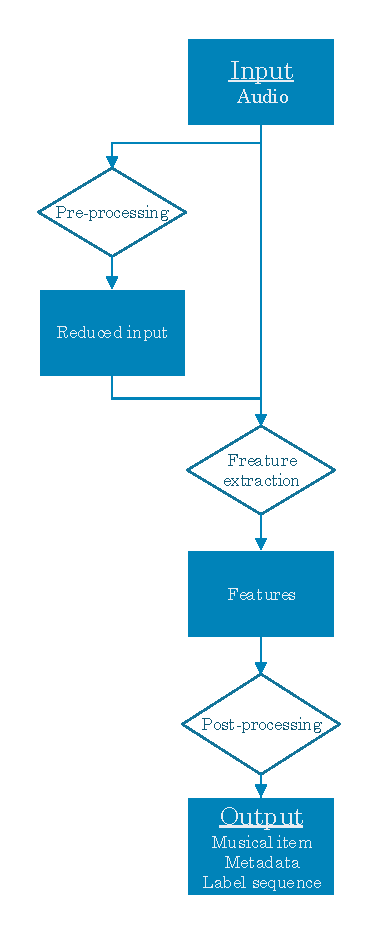
\includegraphics[width = 0.4\linewidth]{obrazky/MIR-diagram.pdf}
    \caption{Řetězec procesů MIR \cite{a_new_companion_to_digital_humanities}}
    \label{fig:MIR_diagram}
\end{figure}

    Digitální hudební nahrávka se jako forma vstupních dat stala hlavním trendem výzkumu \acs{MIR}.
    Je to způsobeno zejména dostupností velkých databází nahrávek ke kterým mají vědecké instituce přístup a nepotýkají se s problémy souvisejícími s autorskými právy \cite{a_new_companion_to_digital_humanities}.

    Z důvodu velké komplexsnosti vstupních dat se využívá několik technik komprimaca signálů. 
    Slučování vícekanálových nahrávek do mono sginálu. Převzorkování signálu na nižší vzorkovací kmitočty,
    a rozložení na krátké překrývající se úseky, ze kterých mohou být nezávisle extrahovány jejich vlastnosti\cite{lidy09:448[TUW-181186]}. 
    Výsledkem je kolekce paralelně složených sekvencí hodnot vlastností, které se následně zpracují na požadovaná výstupní data.

  \begin{table}[H]
    \centering
    \begin{tabular}{|p{0.07\linewidth} | p{0.31\linewidth} | p{0.27\linewidth} | p{0.25\linewidth}|}
        \hline
        {\bf Data}                 & {\bf Vyhledávání informací} & {\bf Klasifikace a odhad} & {\bf Sekvenční značení}\\
        \hline
        Audio                      & Indetifikace kopi \uv{coverů},
                                     Řazení skladeb,
                                     Měření podobnosti,
                                     Získání otisku,
                                     Generování seznamu skladeb
                                   & Identifikace umělce a skladatele,
                                     Žánr a nálada,
                                     Určení tempa
                                   & Extrakce melodie,
                                     Odhad akordů,
                                     Detekce nástupů,
                                     Segmentace                   \\
        \hline
    \end{tabular}
    \caption{Typické procesy na základně vstupních a výstupních dat. \cite{a_new_companion_to_digital_humanities}}
    \label{tab:MIR_typicke_procesy}
  \end{table}

  \subsection{Současné problémy}

  %TODO: dopsat kapitolu

  \section{Parametrizace hudebních nahrávek} \label{sec:Parametrizace}
  V této kapitole je popsán audio signál. Jak vzniká, jeho reprezentace v číslicovám zpracování a základní principy práce s audiosignálem.
  V bodech \ref{sec:Dynamika} a \ref{sec:Barva} jsou popsány parametry získávané z audio signálu.
  Získané parametry slouží pro přesnější popis skladby.

  \subsection{Reprezentace audio signálů} \label{sec:Audio}
  Hudba může být reprezentována spoustou forem. 
  Jako tradiční médium pro její ukládání ještě před vznikem záznamu sloužily vždy noty a další typy zápisů pomocí symbolů.
  Výsledné hudební dílo ale představuje mnohem více než počáteční notový zápis.
  Každý hudebník a hudební nástroj do skladby dodává svou unikátnost.
  Při hře se noty začnou proměňovat v harmonické zvuky, hladké melodie a nástroje vzájemně rezonují. 
  Každý z hudebníků do skladby přináší svou interptretaci. Jinak reagují na tempo zvýrazňují odlišné noty a liší se jejich artikulace.
  Všechny tyto proměnné ve výsledku způsobují, že dílo není jen mechanické přehrání napsané partitury.
  Jeho součástí se stává unikátní přednes \cite{fundamental_of_music_processing}.

  Při pohledu z fyzikálního hlediska důsledkem interpretace díla vznikají zvukové vlny šířící se vzduchem.
  Tyto vlny jsou reprezentovány kmítáním částic v pružném prostředí. V takovém prostředí jsou částice na sebe vázány a vytvářejí soustavu oscilátorů. Pokud dojde k vychýlení jedné částice ze své rovnovážné polohy,
  vlivem okolních částic dochází k působení pružných sil a vzniká její kmitání. 
  Zároveň dochází k vzájemnému rozkmitání okolních částit a prostředím se začne šířít vlna. Jednotlivé částice kmitají pouze kolem své rovnovážné polohy. Nedochází tak k přenosu látky ale pouze energie a hybnosti\cite{crocker1998handbook}.
  Popsané kmitání jsme schopní zachytit pomocí akustických měničů.
  Je získán analogový signál šířících se zvukových vln nazývaný jako audio signál.
  Pojmem audio je označován řetězec sloužící k záznamu, přenosu a reprodukci zvuků v mezích lidského slyšení.
  Avšak v audio signálu se už nenachází přesná reprezentace not a jejich paramterů jako jsou čas nástupu, tón, délka trvání, dynamika.
  Díky tomu je analýza hudebních signálů obtížným úkolem a je ovlivněna reprezentací interpreta akustikou prostoru a vnímáním posluchače.
  Zmíněnými problémy se zabývá samostatný vědní obor s názvem psychoakustika.
  Nejdůležitějšími parametry audio signálu které jsou podrobně popsány níže definujeme: frekvence, výška tónu, dynamika, intenzita, hlasitost a také barva \cite{fundamental_of_music_processing}.

  \subsection{Časová oblast}
  Základní reprezentací audio signálu je tzv. zobrazení v \textbf{časové oblasti}.
  V časové oblasti představují číslicový signál vzorky. Jednotlivé vzorky udávají hodnotu signálu v daném čase.
  Počet vzorků vztažených na jednotku času určuje vzorkovací frekvence signálu.
  Důležitým pravidlem pro vzorkování signálu je Shannonův-Nyquistův vzorkovací teorém popsán rovnicí \ref{rov:vzorkovaci_teorem},

  \begin{equation}
    f_{vz} > 2f_{max}
    \label{rov:vzorkovaci_teorem}
  \end{equation}

  kde $f_{vz}$ je vzorkovací frekvence a $f_{max}$ je maximální frekvence v audio signálu \cite{bracewell1978fourier}.  
  Pokud jednotlivé vzorky zobrazíme graficky získáme průběh signálu v čase viz obr.\ref{fig:Waveform}.

  \begin{figure}[H]
    \centering
    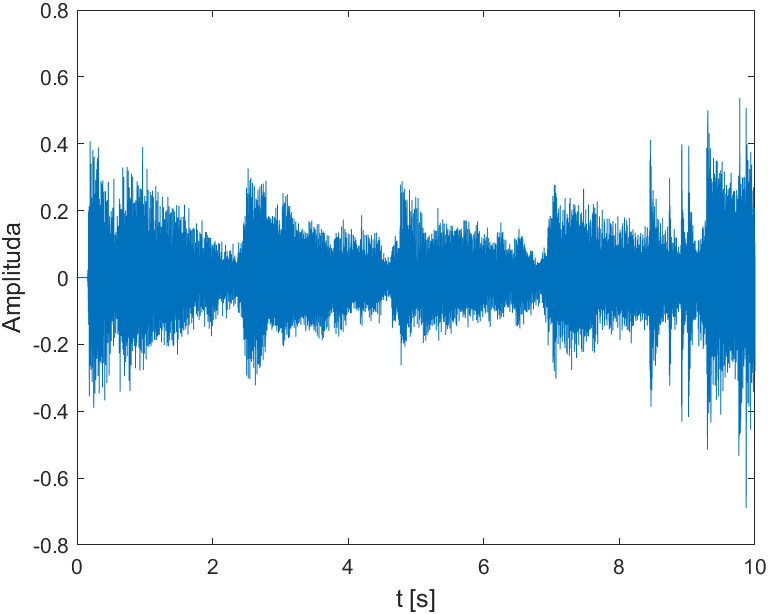
\includegraphics[width = 0.8\linewidth]{obrazky/Waveform.png}
    \caption{Zobrazení časového průběhu signálu}
    \label{fig:Waveform}
  \end{figure}

  Tato reprezentace audio signálu poskytuje informace průběhu amplitudy signálu. Využívá senapříklad pro výpočet energie signálu popsaný v bodě \ref{sec:energie_signalu}.
  
  \subsection{Frekvenční oblast} \label{sec:FFT}
  Pro získání dalalších informací o hudebním díle se využívá transformace signálu do frekvenční oblasti umožňující odlišné znázornění struktury signálu.

  Ve frekvenční oblasti je signál reprezentován jeho frekvenčními složkami popsanými v komplexním tvaru.
  Spektrum představuje rozložení původní části signálu na jednotlivé frekvenční složky popsané funkcí sinus. Kde reálná složka obsahuje informaci o modulu \uv{velikosti} funkce sinus.
  Imaginární složka komplexního čísla pak udává počáteční fázi.
  V grafu jsou poté zobrazy frekvenční složky se kterých se signál skládá viz obr. \ref*{fig:Bass_tone}.

  \begin{figure}[H]
    \centering
    \begin{subfigure}[b]{0.8\linewidth}
        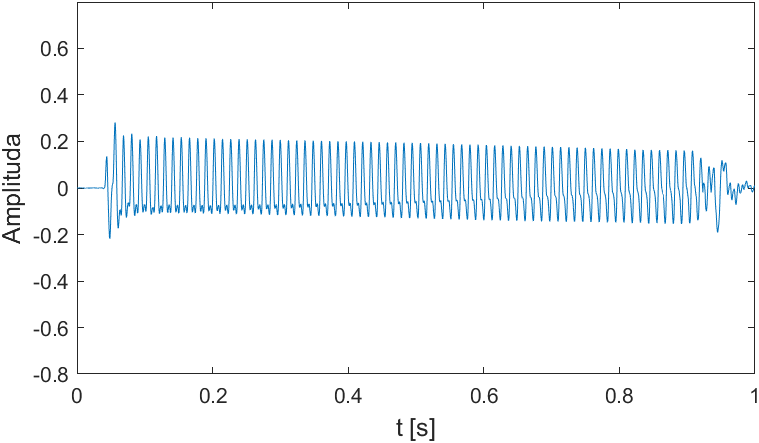
\includegraphics[width = \linewidth]{obrazky/Bass_tone_waveform.png}
        \caption{Časová oblast}
    \end{subfigure}
    \begin{subfigure}[b]{0.8\linewidth}
        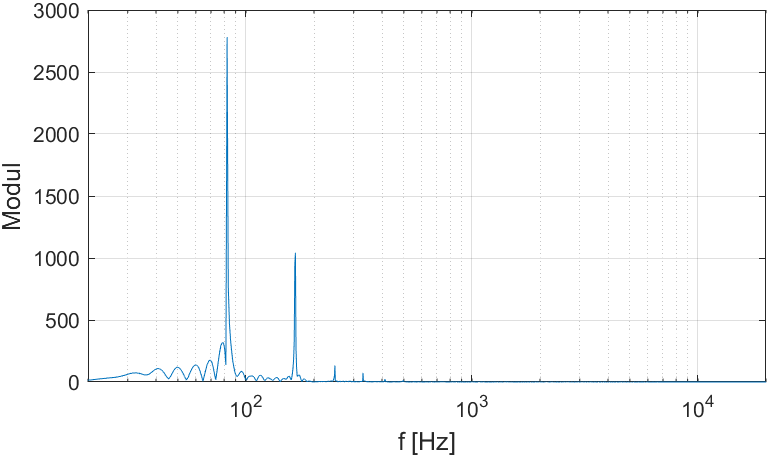
\includegraphics[width = \linewidth]{obrazky/Bass_tone_spectrum.png}
        \caption{Frekvenční oblast}
    \end{subfigure}
    \caption{Reprezentace tónu E zahraného na basovou kytaru.}
    \label{fig:Bass_tone}
\end{figure}
  
  Jako názorný důvod proč je transformace do frekvenční oblasti přínosná je dán příklad. Na nástroj je zahrán tón, který je zaznamenán. 
  V časové oblasti je možné určit délku tónu a jeho průběh podle ADSR obálky popsané v bodě \ref*{sec:Barva}.
  Pokud je ale potřeba zjistit výšku tónu a určit notu, tak se jedná o složýitý proces.
  Díky transformaci do frekveční oblasti je patrná fundementální frekvence tónu.
  Označována také první harmonická.
  Tato frekvence udává výšku tónu a je tak možné stanovit notu která byla zahrána.

  Pro získání frekvenčního spektra signálu je třeba transformovat signál s časové oblasti.
  K tomu se využívá \textbf{Fourierovy transformace}.
  Definována jako transformace převádějící signál mezi časovou a fekvenční oblastní poomcí harmonických signálů \uv{funkce sins a cosinus}.

  Hlavní pilířem Fourierovy transformace je, že každý periodický signál je možné rozložit na součet někonečně mnoha sinusových signálů s různou amplitudou a fází \cite{bracewell1978fourier}.
  Toho je poté pomoí matematickýh postupů docílit.
  Analyzující signál je rozložen na jeho frekvenční složky udávané amplitudou a fází viz obr. \ref*{fig:Bass_tone}.
  Jako další grafické zobrazení frekvenční oblasti hudebního signálu se pro jeho analýzu využívá spektrogramu.
  % Spektrogram zobrazuje frekvenční složky signálu v závislosti na čase. Modul těchto složek je pak udáván barevnou škálou.
  % Spektrogram je zobrazen na obrrázku č. %TODO: popsat spektrogram zde nebo jinde? a popsat? 


  \subsection{DFT - Diskrétní Fourierova transformace} \label{sec:DFT}

\cite{strichartz2003guide}

  Pokud jsou signály zpracovávány pomocí výpočetních procesorů,
  tak může být uložen pouze omezený počet parametrů signálu.
  To znamená, že analogový signál spojitý v čase musí být převeden na signál digitální tvz. signál diskrétní, který je není spojitý v čase. 
  Diskrétní signál je potom vhodný pro číslicové zpracování.
  Důsledkem toho bylo nutné odvodit algoritmus \acs{DFT} přizpůsobený právě pro zpracování diskrétních signálů s konečným počtem hodnot.

  \begin{figure}[H]
    \centering
    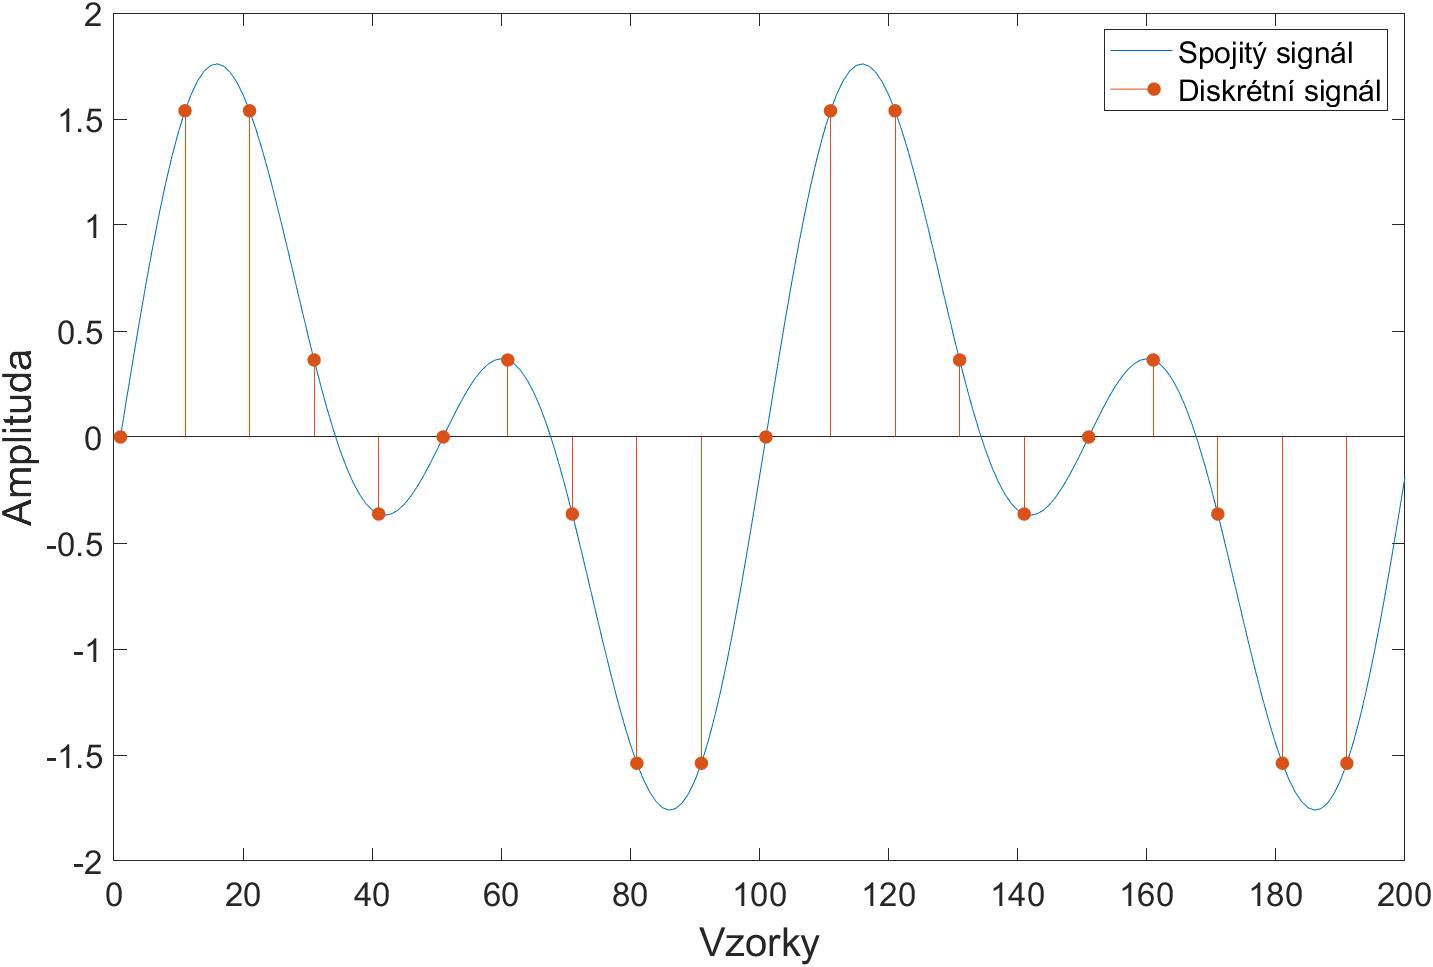
\includegraphics[width = 0.8\linewidth]{obrazky/Discrete_signal.png}
    \caption{Časově spojitý signál a diskrétní signál}
    \label{fig:Discrete_signal}
  \end{figure}

  Rovnice pro \acs{DFT} je potom zapsána v následujícím tvaru. 

  \begin{equation}
    X(k) = \hat{x}(k/N) = \sum_{n = 0}^{N - 1} x(n) exp(-2 \pi i k/N)
    \label{rov:DFT}
  \end{equation}

  Kde $ k \in [0:M - 1] = [0:N - 1] $ a $ M \in \mathbb{N}$.

  Ze strany výpočetní náročnosti je takto definovyný algoritmus neefektivní a výpočetně náročný.
  Při počítání Fourierova koeficientu $X(k)$ je zapotřebí velkého množství velké množství operací v řádu $N^2$.
  Proto pokud počet vzorků $N$ dosahuje většího množství je ve většině případů tento algoritmus příliš pomalý pro praktické využití.

  Počet potřebných operací může být výrazně redukován použitím efektivního algoritmu známého jako \acs{FFT} (\acl{FFT}).
  Na vytvoření\acs{FFT} se zasloužil Carl Friedrich Gauss a Joseph Fourier zhruba před dvěma sty let.
  Vynález tohoto algoritmu změnil své odvětví zpracování signálů a je dnes používán v miliardách telekomunikačních zařízeních.
  Ačkoliv je ve velké míře využíván v telekomunikacích, tak právě i ve zpracování a analýze zvukových signálů zabírá důležitou roli.

  Zjednodušeně \acs{FFT} využívá redundace napříč sinusovými signály různých frekvencní ke společnému výpočtu všech Fourierových koeficientů pomocí rekurze.
  Díky tomu je dosaženo snížení výpočetní náročnosti počtu operací z řádu $N^2$ na $N\log_2 N$.
  Například při použití vzorků $N = 2^10 = 1024$. \acs{FFT} vzžaduje $N\log_2N = 10240 $ operací namísto
  $N^2 = 1048576$ operací při použití \acs{DFT}. Jak je vidět snížení výpočetní náročnosti je velké a exponenciálně roste s větším počtem vzorků $N$.
  
  \subsection{STFT - Short-time Fourier transform} \label{sec:STFT}

  V roce 1946 Dennis Gabor představil \acs{STFT} jako potřebu zařazení frekvenčních složek do konkrétnímo času signálu.
  Fourierova transformace umožňovala převod signálu z časové oblasti do frekvenční ale nebylo zřejme v jakém časovém úseku signálu se získané fekvenční složky nachází.
  Hlavní myšlenkou \acs{STFT} je, že namísto analyzování celého signálu je signál analyzována pouze jeho malá část.
  Za tímto účelem je definována tzv. okénokvá funkce, která je nenulové pouze v malé části signálu.
  Analyzovaný signál je následně vynásoben vzniklou okénkovou funkcí a díky tomu vzniká malá nenulová části signálu dle okénkové funkce viz obr. \ref{fig:princip_stft}.
  Chceme li analyzovat signál v různých časech je tato funkce po signálu posouvána a následně se počítá Fourierova transformace pro každý výsledný okénkový signál.

  \begin{figure}[H]
    \centering
    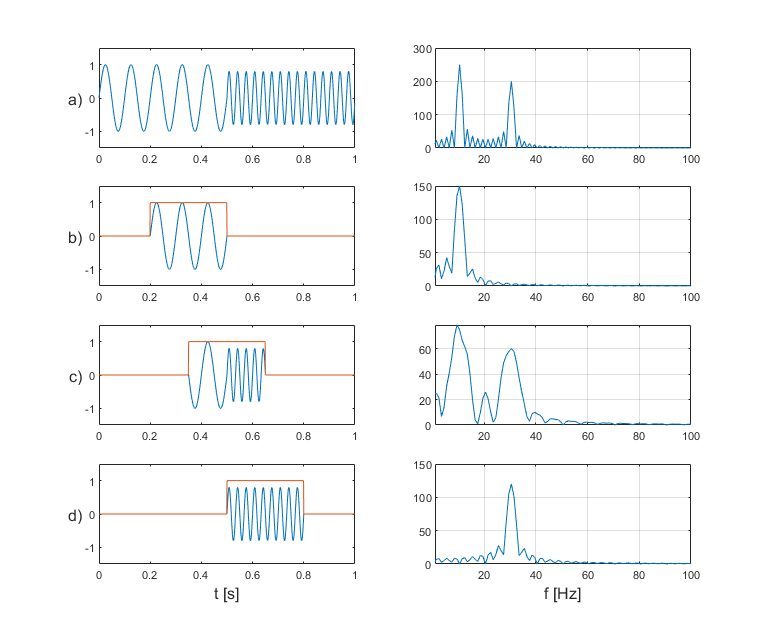
\includegraphics[width = 1\linewidth]{obrazky/STFT.png}
    \caption{Signál o délce $1 s$ s počáteční frekvencí $10 Hz$ a koncovou frekvencí $30 Hz$ \textbf{a)} Původní signál \textbf{b)} Signál s okénkem od $0,2 s$ do $0,5 s$ \textbf{c)} Signál s okénkem od $0,35 s$ do $0,65 s$ \textbf{d)} Signál s okénkem od $0,5 s$ do $0,8 s$};
    \label{fig:STFT}
  \end{figure}

  Na obr. \ref*{fig:STFT} je graficky znázorněna myšlenka \acs{STFT}, která ukazuje výhodu přesného určení frekvenčních složek signálu v čase. 
  Signál je násoben obdelníkovou okénkovou funkcí ve třech místech.
  Tyto tři vzniklé signály jsou následně na sebe nezávazně transformovány do frekvenční oblasti.
  Z výsledků Fourierovy transformace lze vidět, že každá z těchto částí má jiné frekvenční spektrum.
  Pokud by bylo zapotřebí například určit přesný přechod mezi dvěma frekvencemi nacházejícími se v signálu. Lze spřesnit časové měřítko analýzy pomocí délky okénka.
  Tím ale dochází ke zmenšení přesnosti ve frekvenční oblasti.
  
  Na výsledku přesnosti analýzy poomcí \acs{STFT} závisí také tvar použité okénkové funkce.
  V obr. \ref*{fig:STFT} je použito obdélníkového okénka které díky svým ostrým hranám zkresluje výsledek o nechtěné frekvenční složky.
  Existuje více tvarů okénkových funkcí pro odstranění nežádoucích složek.
  Například to jsou Kaise, Chebyshev, Hann a Haming a další.
  \cite{Time-frequency_distributions};

  \subsection{Dynamika hlasitost a intenzita} \label{sec:Dynamika}
  
  V češtině se pojem hlasitost využívá pro reprezentaci subjektivního vnímání akustickho tlaku definovanou například jednotkou phon\footnote{Phon - logaritmická jednotka vyjadřující individuální vnímání hlasitosti. Vnímání hlasitosti lidského ucha je závislé na křivce prahu slyšení a může se lišit pro každý tón \cite{tumarkin_1950}.}. 
  Stejně tak je hlasitost využívána, hovoří li se o měřené hlasitosti vyjádřené například hladinou intenzity zvuku popsanou níže nebo efektivní hodnotou signálu.
  Z důvodu lepší srozumitelnosti jsou dále využívána anglické pojmy \uv{volume} a \uv{loudness}. 

  \textbf{Dynamika} popisuje průběh hlasitosti \uv{volume}interpretovaného hudebního díla. Udává jeden z faktorů jak lze například odlišit stejnou skladbu zahranou různými muzikanty. Interpretací skladby umělec vytváří dynamiku přednášeného díla \cite{fundamental_of_music_processing}.
  V notovém zápise je dynamika neboli hlasitost přednesu popsána symboly jako jsou například pianissimo \uv{\emph{pp}}, piano \uv{\emph{p}}, forte \uv{\emph{f}} a další.

  V audio signálu je dynamika brána jako hlasitost \uv{loudness} Jedná se o změny apmlitudy signálu nebo jeho efektivní hodnoty \acs{RMS}\footnote{RMS - udává statistickou hodnotu z měření velikosti veličin. Je využívána u periodických veličin\cite{RMS_value}.} v čase.

  Při měření hlasitosi \uv{loudness} v akustickém prosotru je pak využíváno pojmů \textbf{intenzita} zvuku a \textbf{akustický výkon}.
  Kde akustický výkon je definovánjako množství energie  vyzářené akustickým vysílačem ve vzduchu za jednotku čausu.\cite{acoustic_power}. Jednotkou je $W$.
  A intenzita zvuku pak je definována jako množství energie, které projde jednotkovou plochou kolmou na směr šíření na jednotku času. Jednotkou pak je $Wm^{-2}$ \cite{intenzita_zvuku_definice}
  
  Z pohledu vnímání hlasitosti lidským uchem je rozsah vnímané intenzity zvuku v řádech bilionů. Práh slyšení činí $10^{-12}$ $Wm^{-2}$ a práh bolesti je $10$ $Wm^{-2}$.
  Pro zmenšení tak velkého řádu je definována hladina intenzity zuvku v decibelech $dB$. Kde vztažnou hodnotou je práh slyšení $I_0 = 10^{-12}$ $Wm^{-2}$.
  Hladina intenzity se vypočítá dle rovnice \ref{rov:hladina_intenzity}.

  \begin{equation}
    L_I = 10*log(\frac{I}{I_0})
    \label{rov:hladina_intenzity}
  \end{equation}

  \subsection{Barva} \label{sec:Barva}

  Hudebním vyjádření se za slovem barva zkrývá velmi komplexní sdružení atributů.
  Jedná se jak o psychologický tak hudební problém který je vnímán individuálně.
  \cite{The_perception_of_musical_timbre}

  Zdjednodušeně se barva definuje jako vlastnosti díky které je možné rozeznat tón o stejné výšce a hlasitosti zahraný na dva různé náastroje.
  Díky barvě je posluchač schopen rozeznávat různé zvuky nástrojů a typů interpretace.

  Jelikož je barva špatně kategorizovatelná fyzikálníma veličinama je většinou interpretována nedefinovanými slovy.
  Například popisujeme barvu jako jasnou, temnou, ostrou, čistou, teplou a další.

  Jedním z možných nástrojů pro analýzu barvy tónu je tvz. obálka tónu/signálu.
  Obálku signálu určuje amplituda signálu v čase viz obr. \ref{fig:ADSR_envelope_on_piano_tone}
  Je rozdělena na 4 fáze a to jsou \textbf{Attack - náběh} určující začátek tónu například úder paličkou na blánu bubnu.
  V této fázi se nachází více ruchových složek z daného úderu a má velkou dynamiku.
  Následuje fáze s názvem \textbf{Decay - útlum}.
  Po hlasitém úderu amplituda signálu klesá a začíná převládat tonální složka. Decay udává dobu za kterou se signál z jeho maxima sníží na hodnotu sustain.
  \textbf{Sustain - podržení} je fáze ve které je zřetelný tón a stálá hlasitost. Rezonující blána bubnu.
  Poslední fází je \textbf{Release - uvolnění} při kterám dochází k poklesu hlasitosti zdroje zvuku až k uplnému utlumení.
  Například přiložení tlumítka na rezonující strunu.

  \begin{figure}[H]
    \centering
    \begin{subfigure}[b]{0.8\linewidth}
        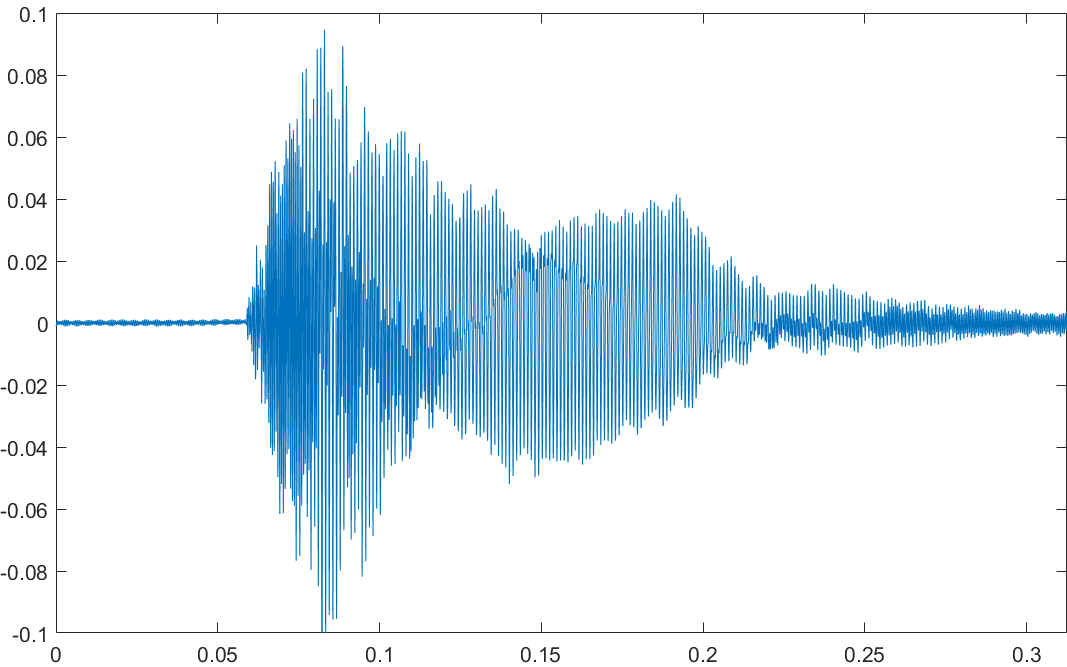
\includegraphics[width = \linewidth]{obrazky/Piano_tone_waveform.png}
        \caption{Amplituda tónu}
    \end{subfigure}
    \begin{subfigure}[b]{0.8\linewidth}
        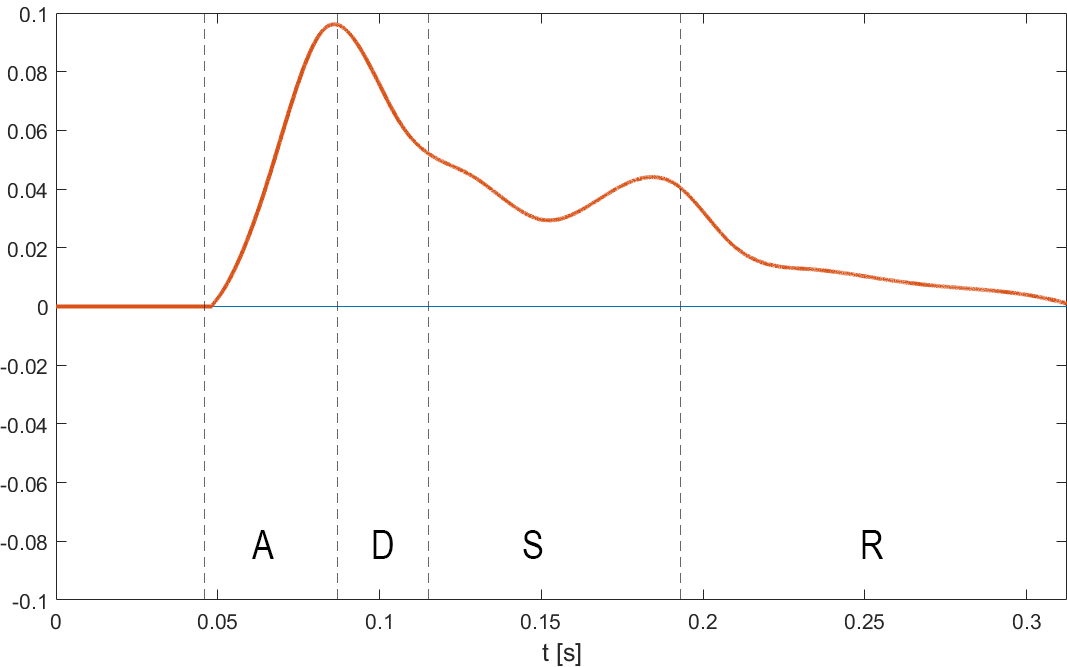
\includegraphics[width = \linewidth]{obrazky/Piano_tone_obalka.png}
        \caption{Obálka tónu}
    \end{subfigure}
    \caption{Tón A5 zahraný na klavír a jeho ADSR obálka}
    \label{fig:ADSR_envelope_on_piano_tone}
  \end{figure}

  Další informace o barvě signálu se nacházejí v jeho frekvenčním spektru. 
  Tón zahraný na hudební nástroj má svou fundamentální (nosnou) frekvenci nazývanou první harmonická frekvence udávající jeho výšku.
  Dle konstrukce nástroje se v signálu objevují násobky nosné frekvence.
  Tyto násobky představují vyšší harmonické složky tónu.
  Počet a amplituda vyšších harmonických složek má velký vliv na výslednou barvu tónu a je to hlavní důvod proč je lidské ucho schopné rozeznat stejný tón znějící na různé nástroje.

  %TODO: vložit obrázek

\section{Detekce dob a analýza tempa skladby} \label{sec:Detekce_tempa}
V této kapitole jsou posány principy detekce tempa skladby a začátků not.
S postupem času se techniky používané v \acs*{MIR} pro detekci dob vyvíjejí a vznikají různé přístupy.
Níže jsou popsány základní principy pro detekci dob a analýzy tempa až po příchod hubokého strojového učení.
Přístup k detekci dob se s vývojem hlubokých neuronových sítí značně změnil. 
Dnes se v této oblasti využívá zejména struktur strojového učení.
\cite{tempobeatdownbeat:book} \cite{fundamental_of_music_processing};

%TODO: popsat problematiku s kapitoly 6.1

  \subsection{Využití energie signálu} \label{sec:energie_signalu}

  \subsection{Využití spektra signálu}
    %TODO: popsat specral flux functio https://tempobeatdownbeat.github.io/tutorial/ch2_basics/baseline.html
  
  \subsection{Detekce periodicity}
    %TODO: popsat autokorelační funkci a její využití pro detekci tempa (periodicity)

  \subsection{Vzužití neuronových sítí}
    Deep neural networks(DNN)
    %TODO: popsat dep learnin při beat trackingu https://tempobeatdownbeat.github.io/tutorial/ch3_going_deep/overview.html
    %TODO: popsat postup (preprocessing, DNN, post processing)/(feature extraction, likelihood estimation, post processing)
  
  \subsection{Více vrstvé perceptronové sítě}

  \subsection{Konvoluční neuronové sítě}
    Temporal Convolutional networks

  \subsection{Rekurentní neuronové sítě}
    Gated recurent units
    Bi-directional models

  \subsection{Hybridní architektury}

\section{Klasifikace žánrů a nálady} \label{sec:Klasifikace_zanru}

\section{"Získání" chromavektorů} \label{sec:Chroma_vektory}

\section{Systém Spectoda} \label{sec:Spectoda}

\section{Hudební signál jako animace}